In order to test the hypothesis, we first derive a number of questions from the hypothesis.
We will also often compare the results on these questions for concept maps to co-occurrence graphs to find differences. While the comparison to co-occurrence graphs is interesting by itself, it is not entirely fair since co-occurrence graphs have far more content than concept maps.

In the next chapter, we will report the results to the experiments we devised to answer the questions which we posed in this chapter and also discuss the significance of the results to our hypothesis.

\todo{Provide the questions that are relevant for the hypothesis}
\todo{What is the best kernel for concept map classification?}
\todo{Extensions to WL?}

\labelsection{Experiments}{subsec:experiments}
To better understand, we devised a number of questions directly concerning our hypothesis.
After finding (approximations to) suitable answers for the posed questions.
In this section we will also introduce the baselines for our tests and describe our methodology in general.
The detailed experiments will be explained more throughly in the next section, alongside the results for the experiments.

Following are the questions we devised in order to understand and test our hypothesis, which is:
\begin{quote}\hypothesis\end{quote}

\todo{Add runtime analysis}

\labelsubsection{Questions}{subsec:questions}

\subquestion{How diverse is the structure of concept maps?}{question:structure_diversity}
When the structure of the graphs is mostly homogeneous or the structural differences are not distinct between graphs of different classes, the structure by itself will most likely not contribute to the classification performance.
When comparing the graph similarity under some graph kernel, the graphs of a given class should be distinguishable from the graphs of the other classes.

To explore the variance in the structure of concept maps, we look at the following metrics:
\begin{enumerate}
    \item{Histogram of the number of connected components}
    \item{Histogram of the size of connected components}
    \item{Average node/edge ratio}
\end{enumerate}

All these methods aim to find out the diversity of the connectedness of concept maps. There a lot of other metrics, but as we will see later on these metrics suffice to get a good picture about the structure of the concept maps.

\subquestion{How important is the structure of concept maps compared to the content?}{question:importance_structure}
Another important question is the relative importance of the structure compared to the content, or the labels.
For this we compare the results of different graph kernels that use \textbf{(a)} only content and \textbf{(b)} only structure and \textbf{(c)} both content and structure.

For the \textbf{content-only kernel}, we will simply count the number of occurrences of labels in the graphs and essentially create a bag-of-words representation of the graph. The kernel then creates the similarity score by calculating the inner product on these vector representations, effectively counting the number of common labels.

For the \textbf{structure-only kernel}, we will use a modified version of the Weisfeiler-Lehman kernel: before executing the WL kernel on the graphs, we first discard all labels on the graph. All nodes of all graphs get the same label. This way, only the structure gets used for the similarity score.

For the \textbf{structure-and-content kernel}, we use the plain Weisfeiler-Lehman graph kernel. 

\todo{We also added an extension to the kernel by using node weights as weights for the labels. We first extracted a weight for each node by calculating the node degree.
We added this extension to give additional weight to label matches of nodes with a greater number of neighbors, ie. higher degree, since matches with a greater neighborhood are far less often.
Instead of the degree, one could also use another metric like PageRank and using the resulting node weights. Using node weights is a trade-off: giving the nodes more weight when they are more connect implies that words that occur often have a high importance!}

\subquestion{How does the classification results of co-occurrence graphs compare to concept maps?}{question:comparison_coo}
For this question, we compare the classification results for concept maps and co-occurrence graphs. As noted before, this comparison is slightly unfair since co-occurrence graphs have far more content than concept maps.
Nevertheless, it is an interesting baseline for graph-based text-classification.

\subquestion{How does the classification performance with concept maps compare to non-structural, text-based approaches?}{question:comparison_text}
Here we test the classification performance of graph-based classification directly with the performance of text-only approaches.
This will give us an insight into the usefulness of concept maps as a text-representation.
This experiment will also serve as a baseline in later experiments.

\subquestion{How useful are multi-word labels in concept maps?}{question:multi_labels}
Concept map node labels often consist of more than one word which is one of the differences to co-occurrence graphs and other graph text-representations.
Yet, our default approach, ie. using Weisfeiler Lehman, does not leverage these multi-word labels.
So, for this question, we evaluate other approaches which make use of the multi-word labels and evaluate the usefulness of them.

\subquestion{How diverse and useful are edge labels in concept maps?}{question:edge_labels}
Another difference of concept maps to co-occurrence graphs is that the former have edge labels.
For this question wee evaluate the importance and role of the edge labels in graph classification. To make use of the edge label, we will also introduce the ``linearized" graph, ie. concept maps converted into text.

\subquestion{Does removing infrequent node labels from the concept map improve classification performance?}{question:infrequent_nodelabels}
As with text, there are often a great number of words which only occur once in the whole dataset. The same applies to concept maps.
In text-based classification approaches, infrequent words are often removed from the text for two reasons: (1) the resulting classifier has less parameters, (2) removing infrequent words greatly reduces the size of feature vectors which, in some cases, can prevent overfitting to too specific features.
Another, WL specific problem is that when a concept only occurs once and it is in the neighborhood of another node, matches in higher iterations of WL are impossible since the concept only occurs once and can not be in any other neighborhood apart from the only occurrence.
For this question, we will evaluate whether removing infrequent node labels will result in better scores.

\subquestion{How does the performance of using the directed edges in concept maps compare to undirected edges?}{question:directed_vs_undirected}
Concept maps, in contrast to co-occurrence graphs, also have directed edges.
To test the effect of using directed versus un-directed edges, we evaluate the classification performance for both cases.

\subquestion{How does the size of concept maps relate to classification performance?}{question:concept_map_size}
The size of a concept map, ie. the number of nodes and edges, is correlated to the size of its underlying text.
Also, the number of occurrences of a single concept in a given text is important for the degree of the corresponding node, ie. when a concept occurs only once in a given text, the corresponding node in the concept map will have a low degree.
On the other hand, when a concept occurs multiple times in a text, the degree of this concept will most likely increase.
These observations give rise to the question whether the size of the concept maps is correlated with the classification performance.
In this experiment we look at the classification scores of concept maps created from texts with varying length.

\subquestion{How different are the datasets and how does it affect the classification performance?}{question:dataset_diversity}
The datasets we chose vary greatly in a lot of ways, some consisting of texts which are informal and written by internet users in online forums while other texts are written by journalists for newspapers.
Other texts are small, others are long.
For this question we evaluate the differences of all theses datasets which hopefully can give insights into the varying relative classification performance of our approaches on different datasets.

\subquestion{How useful are the concept maps combined with text classification?}{question:comparison_combined}
This question aims to directly answer our hypothesis. 
When concept maps indeed have a structure that is useful for classification and which is not captured by text-only approaches, the classification performance should increase when combining graph- and text based approaches.
We test the performance of the combined text- and graph features by concatenating the vectors of both approaches and then training a classifier with these vectors.
We also compare the results with both text-only and graph-only approaches.

\subquestion{How does the compute time of graph-based- compare to text-based  approaches?}{question:comparison_runtime}
Another important question concerns the complexity of our approach.
While graph kernels like Weisfeiler-Lehman or the Random-Walk kernel have seen a rise in efficiency and improvement in runtime, there is still an overhead associated with creating concept maps.

\subsection{Baselines}
\paragraph{Preprocessing}
Before creating the vector representations of the text documents or the creation of the co-occurrence graphs and concept maps, we first pre-process the plain text by

\begin{itemize}
\item{lower-casing the text,}
\item{removing non-printable characters,}
\item{replacing numbers with \textit{NUMBER} placeholders,}
\item{replacing tabs and newlines with a space,}
\item{and normalizing the whitespace (eg. replacing multiple spaces with a single space)}
\end{itemize}
These pre-processing steps are similar to the pre-processing done in \cite{Cachopo2007}.
An example of pre-processing can be seen in Figure \ref{fig:preprocessing_example}.

\begin{figure}[htb!]
	\begin{subfigure}[b]{0.45\linewidth}
\noindent\fbox{%
\parbox{\textwidth}{%
\textsf{I've heard *unconfirmed* rumours that there is a new Integra being released
	for '94.
	\\
	\\
	Does anybody have any info on this?
	\\
	\\
	The local sales people know as much as I can throw them.
	\\
	\\
	--Parms.}}}
    \caption{Before}
    \end{subfigure}
\hspace{0.5in}
	\begin{subfigure}[b]{0.45\linewidth}
\noindent\fbox{%
\parbox{\textwidth}{%
\textsf{i've heard unconfirmed rumours that there is a new integra being released for ' NUMBER. does anybody have any info on this? the local sales people know as much as i can throw them. parms.}}}
\vspace{0.5in}
    \caption{After}
    \end{subfigure}
	\caption[Example: Pre-Processing]{Pre-processing example. Text taken from \textit{ng20} dataset.}\label{fig:preprocessing_example}
\end{figure}

For the co-occurrence graphs, we also optionally filtered out the non-nouns to increase the compression and thus achieve more comparability to concept maps.

\paragraph{Text-based representations}
For the text classification pipeline, we used two different text vectorization algorithms, namely
\begin{itemize}
\item{\textit{Bag Of Words} (BoW): this algorithm simply gathers all words in the corpus and creates a mapping between words and consecutive indices. Then it creates a vector representation for each text so that the i-th vector component is the count of the corresponding word in the text. Ie. $i$ is the index of the word in the mapping.}
\item{\textit{Term-Frequency-Inverse-Document-Frequency} (TfIdf): this approach is an extension to BoW. Instead of using only the counts of a word in the text, this approach also incorporates the term frequency and the inverse document frequency of the words into the vector representation.}
\end{itemize}
Both approaches can also be extended by not only utilizing single words (unigrams) but n-grams, too. A word n-gram consists of $n$ words that appear consecutively in the text.
For example, the sentence ``This is a sentence." has the following 2-grams, or bigrams: $\{ (This, is), (is, a), (a, sentence) \}$.
For our purposes, we looked at both unigrams and bigrams.
Note that word n-grams do not take word inversion into account, ie. the bigram (a, b) is not the same as (b, a).

\paragraph{Graph-based representations}
To compare the performance of concept maps with other graphs, we generated co-occurrence graphs with window sizes $w \in \{1, 2, 3, 4\}$.
We also evaluated the performance of co-occurrence graphs where only nouns are retained to mimic the compression factor of concept maps.

For the extraction of the concept maps from the text, we used the implementation by Falke, introduced in \cite{Falke2017}.
An explanation of the steps to create the concept maps is given in \ref{sec:implementation}.
\todo{Directed edges!}

\begin{figure}[htb!]
\centering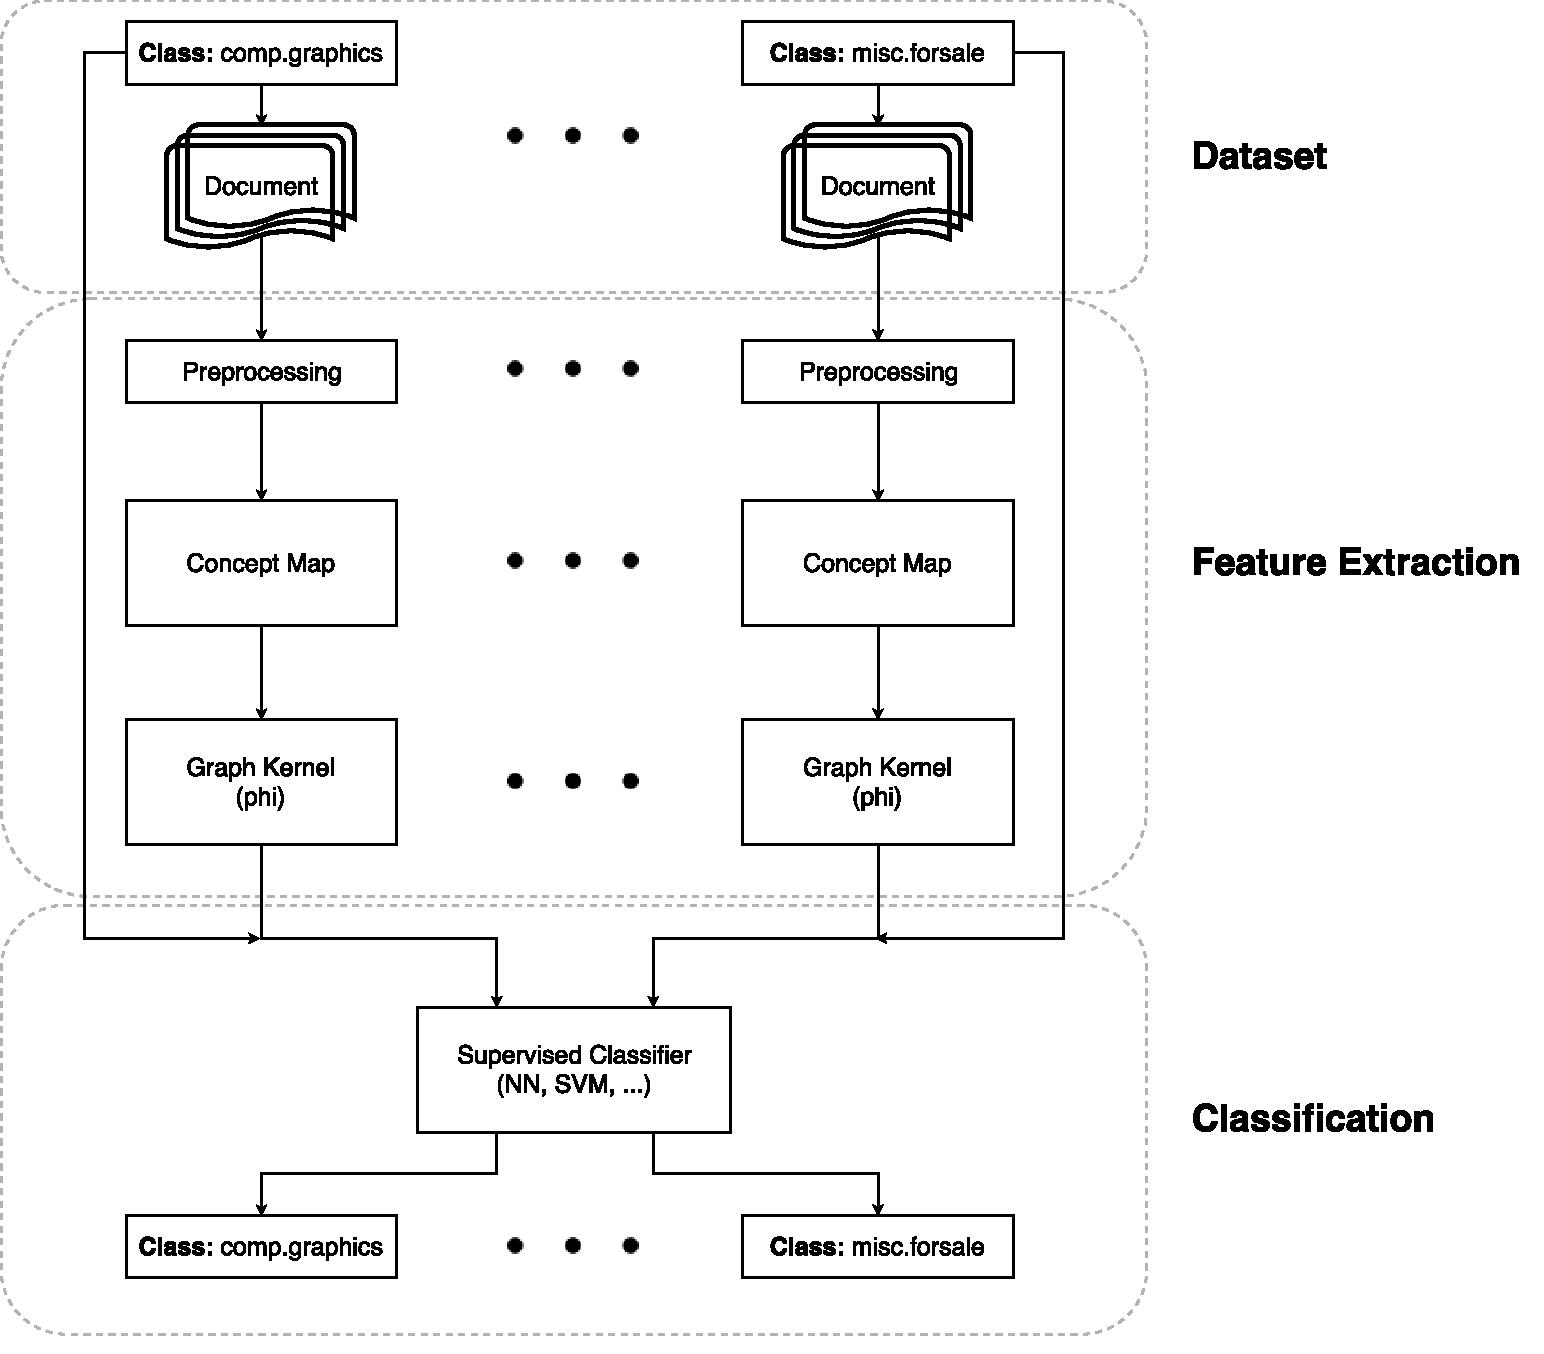
\includegraphics[width=0.6\linewidth]{assets/figures/approach.pdf}
\caption[Diagram: Graph kernel based classification]{Graph kernel based classification pipeline.}
\end{figure}
\todo{Add diagram for gram-matrix based classification.}

\labelsection{Datasets}{subsec:datasets}
We chose a number of datasets, ranging from informal texts written by internet users, eg.  the \textit{ng20} internet forum corpus, to more structured texts, eg. the \textit{nyt} corpus.
The texts of the corpora are also of varying length, enabling us to evaluate the effect of varying concept map sizes.

We provide download links for all the datasets except for the commercial \textit{nyt} dataset.
A script to download these datasets is also provided alongside the other code.

\paragraph{ling-spam}
The Ling-Spam dataset was created and introduced by Androutsopoulos et al. in  \cite{Androutsopoulos2000}.
The corpus contains email texts which are categorized as ``spam" and ``no spam".
One thing to note is that the classification scores with standard methods are quite high by default, so most likely no substantial increase in performance is to be expected.

We obtained a copy of the corpus from here \footnote{\url{http://csmining.org/index.php/ling-spam-datasets.html}}.


\paragraph{ng20}
The 20 Newsgroup corpus consists of posts from an internet forum and was introduced in \cite{Lang}. Each post is labelled with one of 20 different classes, corresponding to the topic it have been posted on. The texts are mostly informal and consist of discussions between users of the forum.
For this dataset, as an additional pre-processing step, we remove the headers and footers from the documents.

While the classes are nearly evenly distributed, some classes are highly correlated\footnote{\url{http://qwone.com/~jason/20Newsgroups/}}, ie. instances of one class A are very similar to the texts from another class B. This adds an additional difficulty to the task.

We obtained the ng20 corpus from here\footnote{\url{http://scikit-learn.org/stable/modules/generated/sklearn.datasets.fetch\_20newsgroups.html\#sklearn.datasets.fetch_20newsgroups}}.

\paragraph{nyt}
The documents in this dataset are articles published in the \textit{New York Times} newspaper in the time between 1987 and 2007.
In total it contains about 1,8 million articles, covering a great number of topics.
Each article has different attributes, examples ranging from the publish date, the author or the section where the article was posted on the \textit{New York Times} website.
As labels we used the online sections an article has been posted to.

We found this dataset when searching for a corpus consisting of long documents. 
For our purposes we only used articles with more than 3000 words and from the six most frequent labels.
Since the extraction of concept maps for documents of this document size takes a long time, we randomly selected 200 documents for each of the six labels, resulting in a dataset of 1200 articles.
Besides the long texts, the other reason we chose this dataset is that it contains high-quality texts.
The texts of most of other datasets we considered are gathered from posts by internet users and often lack basic punctuation or contain misspellings.
This missing structure makes the extraction of concept maps harder since they concept map extraction relies on reliable part-of-speech tags which in turn profit from correct spelling and syntax. 

We obtained our copy of the dataset from here\footnote{\url{https://catalog.ldc.upenn.edu/LDC2008T19} (This is a commercial dataset and has to be bought.)}.

\paragraph{reuters-21578}
This dataset consists of news articles collected and published by Carnegie Group and Reuters.
 The class distribution of the \textit{reuters-21578} dataset is highly skewed, ie. the number of instances per class is not the same for all classes.
 Some of the articles have multiple classes assigned. For our purposes, that is single-label classification, we only used articles with one class.
 We also only use documents which consist of more than 20 words, so that meaningful concept maps can be created.

We obtained the \textit{reuters-21578} dataset from here\footnote{\url{http://www.nltk.org/book/ch02.html\#reuters-corpus}}.

\paragraph{r8}
This dataset is a subset of the \textit{reuters-21578} dataset.
It consists of the 8 most frequent classes of the \textit{reuters-21578} dataset, ie. the 8 classes with the most documents.

\paragraph{review\_polarity}
The \textit{review\_polarity v2} dataset consists of positive and negative reviews for movies by users.
One thing to note is that these reviews are often quite short and informal.

The dataset was introduced in \cite{Pang2004}. We obtained our copy from the author's website \footnote{\url{http://www.cs.cornell.edu/people/pabo/movie-review-data/review\_polarity.tar.gz}}.

\paragraph{rotten\_imdb}
This dataset consists of sentences, each labeled with one of two classes: \textit{subjective} or \textit{objective}.
Note that this dataset consists of short texts and can therefore be used to evaluate the performance of small concept maps.

The dataset w as introduced in \cite{Pang2004}. We obtained our copy from the author's website\footnote{\url{http://www.cs.cornell.edu/people/pabo/movie-review-data/rotten\_imdb.tar.gz}}.

\paragraph{tagmynews}
This corpus consists of summaries obtained from the RSS feeds of three news sites, namely \textit{nyt.com}, \textit{usatoday.com} and \textit{reuters.com}.
The dataset was introduced in \cite{Vitale2012a}.
We obtained the copy from the author's website\footnote{\url{http://acube.di.unipi.it/repo/news.gz}}.	

\paragraph{webkb}
This dataset consists of websites which have been downloaded from 4 american universities. It was collected 1977 during the \underline{W}orld \underline{W}ide \underline{K}nowledge \underline{B}ase project by the CMU Text Learning Group.
The webpages are grouped in seven classes. The distribution of this very skewed, for example with one class having over 3000 instances and another only a little over 100.
We obtained a copy of this dataset from here\footnote{\url{http://www.cs.cmu.edu/afs/cs/project/theo-20/www/data/}}.

\begin{figure}[htb!]
\centering
\begin{tabular}{lrrrr}
{} &  \# classes &  \# docs &  median \#words/doc &  \#uniq. words/\#words \\
\midrule
ling-spam       & 2 & 2893 & 277 & 0.20 \\
ng20            & 20 & 18846 & 79 & 0.07 \\
reuters-21578   & 90 & 13328 & 94 & 0.07 \\
review\_polarity & 2 & 2000 & 589 & 0.16 \\
rotten\_imdb     & 2 & 10000 & 19 & 0.34 \\
tagmynews       & 7 & 32600 & 24 & 0.11 \\
webkb           & 7 & 8274 & 158 & 0.15 \\
\bottomrule
\end{tabular}
\caption[Statistics: Datasets]{Dataset statistics.}
\end{figure}

\labelsection{Methods}{subsec:methods}

\subsection{Cross-Validation}
For all the classification tasks we used train-/validation- and test sets.
The split is done as follows: 85\% for train- and validation set together and 15\% for the validation set.
We then use stratified k-fold cross-validation to further split the train- and validation set. In our case, we used $k = 3$, meaning that $\frac{2}{3}$ of the dataset is used for training, and the rest for validation.
The stratification ensures that the class distribution in the train set is (nearly) the same as in the validation set.

\todo{Hold-out set!}

\subsection{Metrics}
We evaluated a number of metrics for each classification task, namely: 
recall, precision, accuracy and the F1-score. We mostly focus on the F1 macro score since it captures the overall performance of classification algorithms by merging two other metrics, namely precision and recall.
For an overview and definition of the mentioned metrics, please see Section \ref{subsec:classification_task}.

\subsection{Significance tests}
When comparing two models we used the permutation test, or exact test, to test the significance of the difference in performance of these two approaches.
The permutation test tests whether the observed difference of the performances of the two approaches is the product of chance.
The test only returns a probability for observing a given performance difference. The test does not give a definite answer whether the difference was due to chance.
When the probability of observing the difference by chance is below a given threshold, we say that the test shows that the approaches really differ in their performance.

Following is an example of a permutation test.

\paragraph{Example}
In this example we will use the permutation test to test whether the 
  performances of two given classifiers, Model A and B, differ in a non-random way.
In Figure \ref{fig:example_permutation_test} we depicted the steps in the permutation test. 
In our example, the hypothesis is that Model A has a lower performance than Model B.
For this example we chose accuracy as the score metric.
To calculate the accuracy, we need the true labels of the dataset, seen in Figure \ref{fig:example_permutation_test} \textbf{\subref{fig:permutation_test_true}}.
In Figure \ref{fig:example_permutation_test} \textbf{\subref{fig:permutation_test_model_predictions}} we see the predicted labels of the two models and the accuracy as a score beneath them. 
We also see the difference in the scores.
In Figure \ref{fig:example_permutation_test} \textbf{\subref{fig:permutation_test_model_predictions}} we also see that Model A has a lower score than Model B.
This lower score could be due to chance and not because Model B is fundamentally better than Model A.
To test our hypothesis more throughly we now execute the permutation test.
In the first step, Figure \ref{fig:example_permutation_test} \textbf{\subref{fig:permutation_test_samples}}, we generate $n$ samples by interchanging the predictions of the two models randomly.
Here, we depicted three randomly selected samples from the $n$ generated samples.
To generate a sample, we switch the predictions of Model A and B for every document with a probability of 0.5.
The switch of two predictions is marked with a red arrow in our depiction.
In the optimal case, one could generate all possible permutations of the predictions, ie. generate all possible samples.
Unfortunately this often is not an option due to the sheer number of possibilities. That said, generating a large number of samples also gives a good basis for judgment.
In the next step, we calculate the accuracy scores for both models for each of the $n$ samples and also calculate the difference between these scores.
In Figure \ref{fig:example_permutation_test} \textbf{\subref{fig:permutation_test_distribution}} we see the histogram of score differences in the samples.
The red lines mark the initially observed difference between the models A and B (also it's negative).
In the last step, we gather these differences and count the number of samples, $n_{higher}$, where the absolute difference between the models is smaller than the score difference of the original predictions of Model A and B.
$n_{higher}$ divided by the total number of generated samples, $n$, is then the frequency of samples, $f_{higher} = \frac{n_{higher}}{n}$, where the score difference was higher when randomly exchanging the predictions compared to the original observed score difference.
$f_{higher}$ gives an intuition about the likelihood of observing the difference between the scores of Model A and B.
In the histogram of observed differences Figure \ref{fig:example_permutation_test} \textbf{\subref{fig:permutation_test_distribution}} this $f_{higher}$ corresponds to the ratio between the area of elements in the blue surface to total area of the histogram.
In our example, $f_{higher}$ is 0.135, meaning that the probability to observe the score difference we see between the two models is 13.5\% when randomly exchanging the predictions of the two models.
This is far too high to accept the hypothesis on ground of these predictions.

\todo{What confidence interval did we choose?}
\todo{\url{https://stats.stackexchange.com/questions/104040/resampling-simulation-methods-monte-carlo-bootstrapping-jackknifing-cross}}

\begin{figure}[htb!]
  \begin{subfigure}[t]{0.29\linewidth}
  \centering
  {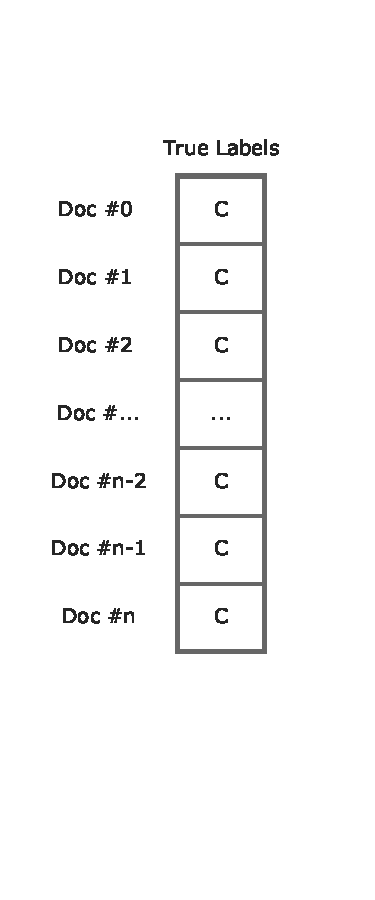
\includegraphics[height=2.2in]{assets/figures/permutation_test/true_labels.pdf}\label{fig:permutation_test_true}}
  \caption{True labels}
  \end{subfigure}
  \hfill
  \begin{subfigure}[t]{.29\linewidth}
  \centering
  {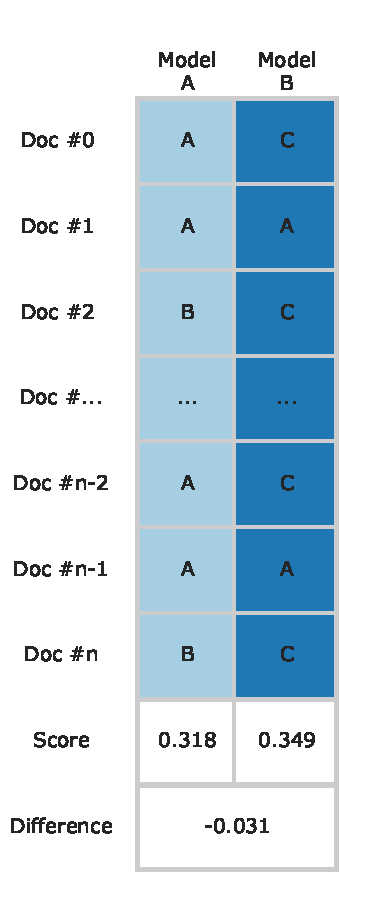
\includegraphics[height=2.2in]{assets/figures/permutation_test/initial_predictions.pdf}\label{fig:permutation_test_model_predictions}}
  \caption{Predictions}
  \end{subfigure}
  \hfill
  \begin{subfigure}[t]{0.40\linewidth}
  \centering
  {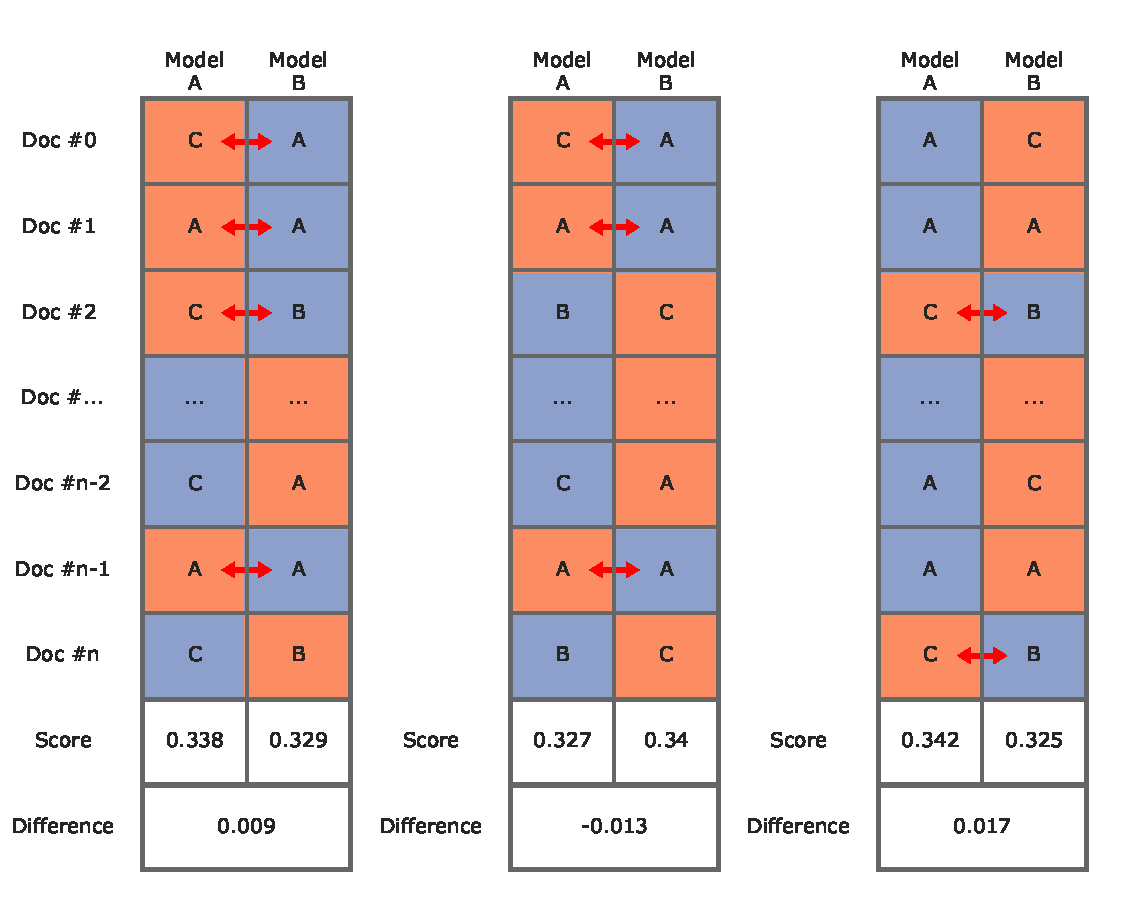
\includegraphics[height=2.2in]{assets/figures/permutation_test/samples.pdf}\label{fig:permutation_test_samples}}
  \caption{Samples}
  \end{subfigure}
  \begin{subfigure}[t]{\linewidth}
  {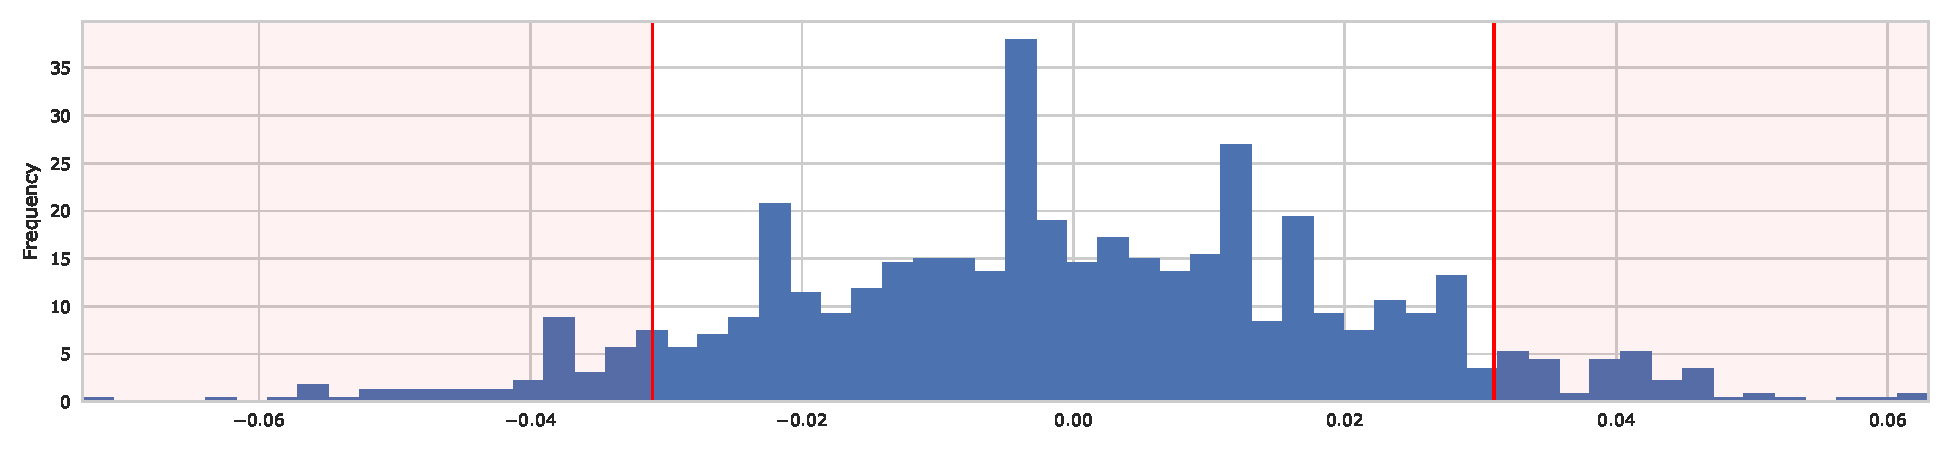
\includegraphics[width=1\textwidth]{assets/figures/permutation_test/distribution.pdf}\label{fig:permutation_test_distribution}}
  \caption{Observed differences in sample scores}
  \end{subfigure}
  \caption[Example: Permutation Test]{Permutation test example. A significance test is most often used to test whether an observed difference is a product of chance or indeed is significant. Significance tests only provide a probability, not a definite answer.}
  \label{fig:example_permutation_test}
\end{figure}


\labelsection{Implementation}{sec:implementation}
We mostly used Python to implement most of the code required to run the experiments.
The code and instructions on how set-up the experiments can be found on GitHub \footnote{\url{https://github.com/davidgengenbach/bachelor-thesis}}.
\todo{Scikit-learn, networkx, \dots}
\todo{Code by Tobias to extract concept maps}

\subsection{Concept Map Extraction}
We used the code \footnote{\url{https://github.com/UKPLab/ijcnlp2017-cmaps}} provided by Falke \cite{Falke2017} to create the concept maps.
In this section we will briefly describe the steps the code performs. For a more detailed explanation, see \cite{Falke2017}.

The input to the concept map extraction algorithm is a single text document. The output is a single concept maps for this text document.

First, the algorithm extracts concepts and their relations to another.
This is done by extracting binary relations from the text. A binary relation consists of three parts: two concepts and the relation between them. An example for a binary relation is ``David likes something", here ``David" and ``something`` are the concepts and ``likes" the relation them. Note that the binary relation is directed, eg. ``Something likes David" is not the same binary relation as ``David likes something."
Also, a concept can consist of multiple words, eg. for ``David likes something else.", the concepts would be ``David" and ``something else".
The extracted concepts are later used as node labels, and the relation between them as the edges between concepts.

Next, the extracted relations get filtered so that only concepts are kept which contain at least one noun and which consist of fewer words than some a given threshold, in our case 10 words. This filtering is done to ensure the brevity and usefulness of the concepts.
\todo{This is somewhat similar to the original text, how to cite?}
